
\item A point travels along the \( x \) axis with a velocity whose projection \( v_x \) is presented as a function of time by the plot in Fig. 1.3.
    \begin{center}
        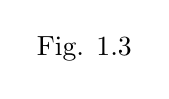
\begin{tikzpicture}
            % Since I cannot create the actual diagram, I'm placing a placeholder here.
            % You will need to replace this with the actual LaTeX/TikZ code for the diagram.
            \node at (0, 0) {Fig. 1.3};
        \end{tikzpicture}
    \end{center}
    Assuming the coordinate of the point \( x = 0 \) at the moment \( t = 0 \), draw the approximate time dependence plots for the acceleration \( w_x \), the \( x \) coordinate, and the distance covered \( s \).
